%% LyX 2.3.7 created this file.  For more info, see http://www.lyx.org/.
%% Do not edit unless you really know what you are doing.
\documentclass[english]{article}
\usepackage{lmodern}
\renewcommand{\sfdefault}{lmss}
\usepackage{courier}
\usepackage[T1]{fontenc}
\usepackage{graphicx}
\usepackage[latin9]{inputenc}
\usepackage{geometry}
\geometry{verbose,tmargin=0.8in,bmargin=0.8in,lmargin=1in,rmargin=1in,headheight=0cm,headsep=0cm}
\usepackage{babel}
\usepackage{array}
\usepackage{amsmath,amssymb,amsthm,latexsym,paralist}
\usepackage{fancyhdr}
\newtheorem*{solution}{Solution}
\usepackage[unicode=true]
 {hyperref}

\makeatletter

%%%%%%%%%%%%%%%%%%%%%%%%%%%%%% LyX specific LaTeX commands.
\providecommand{\LyX}{\texorpdfstring%
  {L\kern-.1667em\lower.25em\hbox{Y}\kern-.125emX\@}
  {LyX}}
%% Because html converters don't know tabularnewline
\providecommand{\tabularnewline}{\\}

%%%%%%%%%%%%%%%%%%%%%%%%%%%%%% Textclass specific LaTeX commands.
\newenvironment{lyxcode}
	{\par\begin{list}{}{
		\setlength{\rightmargin}{\leftmargin}
		\setlength{\listparindent}{0pt}% needed for AMS classes
		\raggedright
		\setlength{\itemsep}{0pt}
		\setlength{\parsep}{0pt}
		\normalfont\ttfamily}%
	 \item[]}
	{\end{list}}

\makeatother

\usepackage{listings}
\renewcommand{\lstlistingname}{Listing}

\begin{document}
\begin{center}
{\Large{}CSCE 221 Cover Page\smallskip{}
}{\Large\par}
\par\end{center}

\begin{center}
{\large{}Manas~~~~~~~~~~~~~~~~~~Navale ~~~~~~~~~~~~~~~~~~~~~333006797~~~~~~~~~~~~~~\bigskip{}
}{\large\par}
\par\end{center}

\begin{center}
{\large{}msn0083-tamu ~~~~~~~~~~~~~~~~~~~msn0083@tamu.edu~~~~~~~~~~~~~~~~~~~~~~~~~~~~~~}\medskip{}
\par\end{center}
\begin{quotation}
Please list all sources in the table below including web pages which
you used to solve or implement the current homework. If you fail to
cite sources you can get a lower number of points or even zero, read
more: \href{http://aggiehonor.tamu.edu/}{Aggie Honor System Office}
\medskip{}
\medskip{}
\end{quotation}
\begin{center}
\begin{tabular}{|c|c|c|c|}
\hline 
Type of sources  & ~~~~~~~~~~~~~~~~~~~~~~~~~~~~~ & ~~~~~~~~~~~~~~~~~~~~~~~~~~~~~~~~ & ~~~~~~~~~~~~~~~~~~~~~~~~~~~~~~~~~\tabularnewline
 &  &  & \tabularnewline
 &  &  & \tabularnewline
\hline 
\hline 
People &  &  & \tabularnewline
 &  &  & \tabularnewline
 &  &  & \tabularnewline
\hline 
Web pages (provide URL)  & https://flexiple.com/algorithms  & https://algorithmtutor.com/Analysis-of-Algorithm/ & \tabularnewline
 & /big-o-notation-cheat-sheet  & Running-Time-Growth-of-Function-and-Asymptotic-Notations/ & \tabularnewline
 &  &  & \tabularnewline
\hline 
Printed material &  &  & \tabularnewline
 &  &  & \tabularnewline
 &  &  & \tabularnewline
\hline 
Other Sources  &  &  & \tabularnewline
 &  &  & \tabularnewline
 &  &  & \tabularnewline
\hline 
\end{tabular}
\par\end{center}

\medskip{}

\begin{quotation}
I certify that I have listed all the sources that I used to develop
the solutions/codes to the submitted work.

\textquotedblleft \emph{On my honor as an Aggie, I have neither given
nor received any unauthorized help on this academic work.}\textquotedblright{} 
\end{quotation}
\vspace{0.5cm}

\begin{tabular}{cccccc}
Manas Navale  & ~~~~~~~~~~~~~~~~~~~~~~~~~~~ &  & ~~~~~~~~~~~~~~~~~~~~~ & 9/20/23  & ~~~~~~~~~~~~~~~~~~~~\tabularnewline
\end{tabular}\vfill{}

\pagebreak{}
\begin{center}
\textbf{\Large{}Homework 1}{\Large\par}
\par\end{center}

\begin{center}
\textbf{\large{}Check the Canvas calendar for the deadliness. }\\
\textbf{\large{}The homework submission to Gradescope only.}{\large\par}
\par\end{center}
\begin{quote}
\textbf{Typeset your solutions to the homework problems listed below
using \LaTeX{} (or \LyX ). See the class webpage for information about
their installation and tutorials.}
\end{quote}
\noindent \begin{flushleft}
\textbf{Homework 1 Objectives:}
\par\end{flushleft}
\begin{enumerate}
\item Developing the C++ programming skills by using
\begin{enumerate}
\item templated dynamic arrays and STL vectors
\item tests for checking correctness of a program.
\end{enumerate}
\item Comparing theory with a computation experiment in order to classify
algorithm.
\item Preparing reports/documents using the professional software \LaTeX{}
or \LyX .
\item Understanding the definition of the big-O asymptotic notation.
\item Classifying algorithms based on pseudocode.
\end{enumerate}
\noindent \begin{flushleft}
\rule[0.5ex]{1\columnwidth}{1pt}
\par\end{flushleft}
\begin{enumerate}
\item (25 points) Include your C++ code in the problem solution\textemdash \textbf{do
not use attachments or screenshots.}
\begin{enumerate}
\item (10 points) Use the STL class \texttt{vector<int>} to write two C++
functions that return true if there exist \textbf{two} elements of
the vector such that their \textbf{product} is divisible by 12, and
return false otherwise. The efficiency of the first function should
be $O(n)$ and the efficiency of second one should be $O(n^{2})$
where $n$ is the size of the vector.
~\\
\begin{lstlisting}[language={C++},basicstyle={\small\ttfamily},showstringspaces=false]
   //first function
   bool LinearFunction(const vector<int>& nums) {
      unordered_set<int> seen;
      for (int num : nums) {
          if (num % 12 == 0 || seen.count(12 - (num % 12)) > 0) {
              return true;
          }
          seen.insert(num % 12);
      }
      return false;
  }

//second function 
bool QuadFunction(const vector<int>& nums) {
    int n = nums.size();
    for (int i = 0; i < n; i++) {
        for (int j = i + 1; j < n; j++) {
            if ((nums[i] * nums[j]) % 12 == 0) {
                return true;
            }
        }
    }
    return false;
}

   \end{lstlisting}
   {\small\par}
\pagebreak
\item (6 points) Justify your answer by writing the running time functions
in terms of $n$ for both the algorithms and their classification
~\\
\\The first function has a running time function of $T(n) = O(n)$ and a linear time complexity.
\\The second function has a running time function of $T(n) = O(n^2)$ and a quadratic time complexity.  
\item (2 points) What do you consider as an operation for each algorithm?
~\\An operation in the first algorithm would be the insertion and the checking:
\begin{lstlisting}[language={C++},basicstyle={\small\ttfamily},showstringspaces=false]
   unordered_set<int> seen;
   for (int num : nums) {
       // Insertion operation (O(1) average time complexity)
       seen.insert(num % 12);
   }
   // Checking for an element operation (O(1) average time complexity)
   if (num % 12 == 0 || seen.count(12 - (num % 12)) > 0) {
       return true;
   }
\end{lstlisting}
{\small\par}
~\\ in the second algorithm it would be the nested loops:
\begin{lstlisting}[language={C++},basicstyle={\small\ttfamily},showstringspaces=false]
   int n = nums.size();
   for (int i = 0; i < n; i++) {
      // inner loop  iteratres over pairs of elements in the 'nums' vector. 
       for (int j = i + 1; j < n; j++) {
           //Constant time operation within the inner loop
           if ((nums[i] * nums[j]) % 12 == 0) {
               return true;
           }
       }
   }   
\end{lstlisting}
{\small\par}
\item (2 points) Are the best and worst cases for both the algorithms the
same in terms of big-O notation? Justify your answer. 
~\\
\\In both algorithms, the time complexity does not change based on the input and remain $O(n)$ and $O(n^2)$. So the best and worst cases are the same. 
\\
\item (5 points) Describe the situations of getting the best and worst cases,
give the samples of the input for each case, and check if your running
time functions match the number of operations. 
~\\
\\The best case scenario for the algorithms would be if a pair divisible is found early so something like $[12, 6, 2, 8, 4, 9]$, while the worst case scenario would be $[1, 2, 3, 4, 5, 6]$ where there algorith examines each input without finding a pair divisible by 12.
~\\
\vfill{}
\end{enumerate}
\newpage{}
\item (50 points + bonus) The binary search algorithm problem.
\begin{enumerate}
\item (5 points) Implement a templated C++ function for the binary search
algorithm based on the set of the lecture slides\textit{ ``Analysis
of Algorithms''}.

{\small{}}
\begin{lstlisting}[language={C++},basicstyle={\small\ttfamily},showstringspaces=false]
int Binary_Search(vector<int> &v, int x) {
   int mid, low = 0;     
   int high = (int) v.size()-1;     
   while (low < high) {         
      mid = (low+high)/2;                 
      if (num_comp++, v[mid] < x) low = mid+1;         
      else high = mid;     
   }     
   if (num_comp++, x == v[low]) return low; //OK: found          
   return -1; //not found
} 
\end{lstlisting}
{\small\par}

Be sure that before calling \texttt{Binary\_Search}, elements of the
vector \texttt{v} are arranged in \textbf{ascending} order. The function
should also keep track of the number of comparisons used to find the
num \texttt{x}. The (global) variable \texttt{num\_comp} keeps
the number of comparisons and initially should be set to zero.
{\small{}}
\begin{lstlisting}[language={C++},basicstyle={\small\ttfamily},showstringspaces=false]
#include <iostream>
#include <vector>
using namespace std;

int num_comp = 0;

template <typename T>
int Binary_Search(vector<T> &v, T x) {
    int mid, low = 0;
    int high = static_cast<int>(v.size()) - 1;

    while (low <= high) {
        mid = (low + high) / 2;
        num_comp++;

        if (v[mid] == x) {
            return mid;
        } else if (v[mid] < x) {
            low = mid + 1;
        } else {
            high = mid - 1;
        }
    }
    return -1;
}

int main() {
    vector<int> sorted_vector = {1, 2, 3, 4, 5, 6, 7, 8, 9, 10, 11, 12, 13, 14, 15, 16};
    
    for (int i = 1; i < sorted_vector.size(); i++) {
        if (sorted_vector[i] < sorted_vector[i - 1]) {
            cout << "Not sorted vector." << endl;
            return 1;
        }
    }

    int num1 = 1;
    int num2 = 16;
    int num3 = 8;

    int location1 = Binary_Search(sorted_vector, num1);
    int location2 = Binary_Search(sorted_vector, num2);
    int location3 = Binary_Search(sorted_vector, num3);

    cout << num1 << " found at index " << location1 << ", comparisons: " << num_comp << endl;
    cout << num2 << " found at index " << location2 << ", comparisons: " << num_comp << endl;
    cout << num3 << " found at index " << location3 << ", comparisons: " << num_comp << endl;

    return 0;
}
\end{lstlisting}
{\small\par}
\medskip{}

\item (10 points) Test your algorithm for correctness using a vector of
data with 16 elements sorted in ascending order. An error message
should be printed or exception should be thrown when the input vector
is unsorted.\\
What is the value of \texttt{num\_comp} in the cases when 
\begin{enumerate}
\item the num \texttt{x} is the first element of the vector 
\texttt{v}
~\\ 
~\\ num comp is 1
~\\
\item the num \texttt{x} is the last element of the vector \texttt{v}
\item 
~\\ 
~\\ num comp is 4
~\\
\item the num \texttt{x} is in the middle of the vector \texttt{v} 
~\\ 
~\\ num comp is 3
~\\
\end{enumerate}
What is your conclusion from the testing for $n=16$?
~\\
~\\ My conclusion is that the binary search algorithm performs a small number of comparisons becasue it is capable of narrowing down the search range effectively. 
\medskip{}

\item (10 points) Test your program using vectors of size $n=2^{k}$ where
$k=0,\,1,2,\dots,11$ populated with consecutive increasing integers
in these ranges: $1,\,2,\,4,\,8,\,16,\,32,\,64,\,128,\,256,\,512,\,1024,\,2048$.
Select the num as the last element in the vector. Record the value
of \texttt{num\_comp} for each vector size in the table below. 

\textbf{}%
\begin{tabular}{|>{\centering}p{2cm}|c|c|}
\hline 
Range {[}1,$n${]} & \multicolumn{1}{>{\centering}p{2cm}|}{num } & \multicolumn{1}{>{\centering}p{2cm}|}{num\_comp}\tabularnewline
\hline 
\hline 
{[}1, 1{]} & 1 & 1 \tabularnewline
\hline 
{[}1, 2{]} & 2 & 1 \tabularnewline
\hline 
{[}1, 4{]} & 4 & 2 \tabularnewline
\hline 
{[}1, 8{]} & 8 & 3 \tabularnewline
\hline 
{[}1, 16{]} & 16 & 4\tabularnewline
\hline 
{[}1, 32{]} & 32 & 5 \tabularnewline
\hline 
{[}1, 64{]} & 64 & 6 \tabularnewline
\hline 
{[}1, 128{]} & 128 & 7 \tabularnewline
\hline 
{[}1, 256{]} & 256 & 8 \tabularnewline
\hline 
{[}1, 512{]} & 512 & 9 \tabularnewline
\hline 
{[}1, 1024{]} & 1024 & 10 \tabularnewline
\hline 
{[}1, 2048{]} & 2048 & 11 \tabularnewline
\hline 
\end{tabular}

\pagebreak
\item (5 points) Plot the number of comparisons for the vector size $n=2^{k}$,
$k=0,1,2,\dots,11$. You can use a spreadsheet or any graphical package.
\begin{figure}
   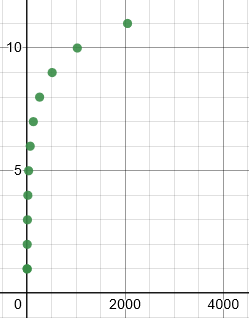
\includegraphics[width = 0.5\textwidth]{Screenshot 2023-09-20 195230.png}
\end{figure}
\item (5 points) Provide a mathematical formula/function which takes $n$
as an argument, where $n$ is the vector size, and returns as its
value the number of comparisons. Does your formula match the computed
output for any input? Justify your answer.

~\\The formula would be $C = \log_2(n)$. The following formula matches the computed output for each input size, except 1, where the number of comparisons was 1, and not 0.  

\medskip{}
\item (5 points) How can you modify your formula/function if the largest
number in a vector is not the exact power of two? Test your program
using input in ranges from $1$ to $n=2^{k}-1$, $k=0,1,2,\dots,11$
and plot the number of comparisons vs. the size of the vector.
~\\ The modified formula would be \(C = \lceil\log_2(n)\rceil\)
\textbf{}%
\begin{tabular}{|c|c|c|}
\hline 
\multicolumn{1}{|c|}{Range {[}1,$n${]}} & \multicolumn{1}{>{\centering}p{2cm}|}{num } & \multicolumn{1}{>{\centering}p{2cm}|}{num\_comp }\tabularnewline
\hline 
\hline 
{[}1, 1{]} & 1 & 0 \tabularnewline
\hline 
{[}1, 3{]} & 3 & 2\tabularnewline
\hline 
{[}1, 7{]} & 7 & 3\tabularnewline
\hline 
{[}1, 15{]} & 15 & 4\tabularnewline
\hline 
{[}1, 31{]} & 31 & 5\tabularnewline
\hline 
{[}1, 63{]} & 63 & 6\tabularnewline
\hline 
{[}1, 127{]} & 127 & 7\tabularnewline
\hline 
{[}1, 255{]} & 255 & 8\tabularnewline
\hline 
{[}1, 511{]} & 511 & 9\tabularnewline
\hline 
{[}1, 1023{]} & 1023 & 10\tabularnewline
\hline 
{[}1, 2047{]} & 2047 & 11\tabularnewline
\hline 
\end{tabular}
\pagebreak
\item (5 points) Do you think the number of comparisons in the experiment
above are the same for a vector of strings or a vector of doubles?
Justify your answer.
~\\
~\\ It would not be the same, as vector of strings, would depend on different variables like the number of characters and the lenght of the string, meaning the comparisons would vary based on input data. For a vector of doubles, it would vary on the specific double value. 
\medskip{}
\item (5 points) Use the big-O asymptotic notation to classify binary search
algorithm and justify your answer.

~\\\textbf{Time Complexity}: \(O(\log_2(n))\)
~\\The key component of this algorithm is the way it reduces the search space in half, and the way the number of comparisons is proportional to the size of the input data. As n grows, the number of comparisons grows(but at a slower rate.)
\medskip{}
\item (Bonus 10 points) Read the sections 1.6.3 and 1.6.4 from the textbook
and modify the algorithm using a functional object to compare vector
elements. How can you modify the binary search algorithm to handle
the vector of descending elements? What will be the value of \texttt{num\_comp}?
Repeat the search experiment for the smallest number in the integer
arrays. Tabulate the results and write a conclusion of the experiment
with your justification. \medskip{}

\newpage{}
\end{enumerate}
\item (25 points) Find running time functions for the algorithms below and
write their classification using big-O asymptotic notation in terms
of $n$. A running time function should provide a formula on the number
of arithmetic operations and assignments performed on the variables
$s$, $t$, or $c$. Note that array indices start from $0$.
\begin{enumerate}
\item \textbf{\small{}Algorithm Ex1(A):}{\small\par}
\begin{lyxcode}
\textbf{\small{}~~Input}{\small{}:~An~array~A~storing~$n\geq1$~integers.}{\small\par}

\textbf{\small{}~~Output}{\small{}:~The~sum~of~the~elements~in~A.}{\small\par}

{\small{}$s\leftarrow A[0]$}{\small\par}

\textbf{\small{}for}{\small{}~$i\leftarrow1$~to~$n-1$~}\textbf{\small{}do}{\small\par}

{\small{}~~~$s\leftarrow s+A[i]$}{\small\par}

\textbf{\small{}end~for}{\small\par}

\textbf{\small{}return}{\small{}~$s$}
\end{lyxcode}
~\\\textbf{Running Time Function}: \(f(n) = n\)
~\\\textbf{Big O}: \(O(n)\)
\item \textbf{\small{}Algorithm Ex2(A):}{\small\par}
\begin{lyxcode}
\textbf{\small{}~~Input}{\small{}:~An~array~A~storing~$n\geq1$~integers.}{\small\par}

\textbf{\small{}~~Output}{\small{}:~The~sum~of~the~elements~at~even~positions~in~A.}{\small\par}

{\small{}$s\leftarrow A[0]$}{\small\par}

\textbf{\small{}for}{\small{}~$i\leftarrow2$~}\textbf{\small{}to}{\small{}~$n-1$~}\textbf{\small{}by~}{\small{}increments~of~2}\textbf{\small{}~do}{\small\par}

{\small{}~~$s\leftarrow s+A[i]$}{\small\par}

\textbf{\small{}end~for}{\small\par}

\textbf{\small{}return}{\small{}~$s$}
\end{lyxcode}
~\\\textbf{Running Time Function}: \(f(n) = \frac{n}{2}\)
~\\\textbf{Big O}: \(O(n)\)
\pagebreak
\item \textbf{\small{}Algorithm Ex3(A):}{\small\par}
\begin{lyxcode}
{\small{}~~~}\textbf{\small{}Input}{\small{}:~An~array~A~storing~$n\geq1$~integers.}{\small\par}

\textbf{\small{}~~~Output}{\small{}:~The~sum~of~the~partial~sums~in~A.}{\small\par}

{\small{}$s\leftarrow0$}{\small\par}

\textbf{\small{}for}{\small{}~$i\leftarrow0$~~}\textbf{\small{}to}{\small{}~$n-1$~}\textbf{\small{}do}{\small\par}

{\small{}~~~$s\leftarrow s+A[0]$}{\small\par}

\textbf{\small{}~~~for}{\small{}~$j\leftarrow1$~}\textbf{\small{}to}{\small{}~$i$~}\textbf{\small{}do}{\small\par}

{\small{}~~~~~$s\leftarrow s+A[j]$}{\small\par}

{\small{}~~~}\textbf{\small{}end~for}{\small\par}

\textbf{\small{}end~for}{\small\par}
\begin{lyxcode}
\textbf{\small{}return}{\small{}~$s$}
\end{lyxcode}
\end{lyxcode}
~\\\textbf{Running Time Function}:\(f(n) = n + \frac{n(n-1)}{2}\)
~\\\textbf{Big O}: \(O(n^2)\)
\item \textbf{\small{}Algorithm Ex4(A):}{\small\par}
\begin{lyxcode}
{\small{}~~~}\textbf{\small{}Input}{\small{}:~An~array~A~storing~$n\geq1$~integers.}{\small\par}

\textbf{\small{}~~~Output}{\small{}:~The~sum~of~the~partial~sums~in~A.}{\small\par}

{\small{}$t\leftarrow A[0]$}{\small\par}

{\small{}$s\leftarrow A[0]$}{\small\par}

\textbf{\small{}for}{\small{}~$i\leftarrow1$~}\textbf{\small{}to}{\small{}~$n-1$~}\textbf{\small{}do}{\small{}~}{\small\par}

{\small{}~~~$s\leftarrow s+A[i]$}{\small\par}

{\small{}~~~$t\leftarrow t+s$}{\small\par}

\textbf{\small{}end~for}{\small\par}

\textbf{\small{}return}{\small{}~$t$}
\end{lyxcode}
~\\\textbf{Running Time Function}: \(f(n) = 2n\)
~\\\textbf{Big O}: \(O(n)\)
\item \textbf{\small{}Algorithm Ex5(A, B):}{\small\par}
\begin{lyxcode}
{\small{}~~~}\textbf{\small{}Input}{\small{}:~Arrays~A~and~B~storing~$n\geq1$~integers.}{\small\par}

\textbf{\small{}~~~Output}{\small{}:~The~number~of~elements~in~B~equal~to~the~partial~sums~in~A.}{\small\par}

{\small{}$c\leftarrow0$~//counter}{\small\par}

\textbf{\small{}for}{\small{}~$i\leftarrow0$~}\textbf{\small{}to}{\small{}~$n-1$~}\textbf{\small{}do}{\small{}~}{\small\par}

{\small{}~~~$s\leftarrow0$~//}\emph{\small{}partial~sum}{\small\par}

\textbf{\small{}~~~for}{\small{}~$j\leftarrow0$~}\textbf{\small{}to}{\small{}~$n-1$~}\textbf{\small{}do}{\small\par}

{\small{}~~~~~~$s\leftarrow s+A[0]$}{\small\par}

\textbf{\small{}~~~~~~for}{\small{}~$k\leftarrow1$~}\textbf{\small{}to}{\small{}~$j$~}\textbf{\small{}do}{\small\par}

{\small{}~~~~~~~~~$s\leftarrow s+A[k]$}{\small\par}

{\small{}~~~~~~}\textbf{\small{}end~for}{\small\par}

{\small{}~~~}\textbf{\small{}end~for}{\small\par}

{\small{}~~~}\textbf{\small{}if}{\small{}~$B[i]=s$~}\textbf{\small{}then}{\small\par}

{\small{}~~~~~~$c\leftarrow c+1$}{\small\par}

{\small{}~~~}\textbf{\small{}end~if}{\small\par}

\textbf{\small{}end~for}{\small\par}

\textbf{\small{}return}{\small{}~$c$}
\end{lyxcode}
~\\\textbf{Running Time Function}: \(f(n) = n + \frac{n^2(n-1)}{2}\)
~\\\textbf{Big O}: \(O(n^3)\)
\end{enumerate}
\end{enumerate}

\end{document}
